\documentclass[11pt,final,oneside]{fithesis}
\usepackage[utf8]{inputenc}
\usepackage[T1]{fontenc}
\usepackage[slovak]{babel}
\usepackage[plainpages=false, pdfpagelabels]{hyperref}
\usepackage{graphicx}
\usepackage{float}
\usepackage{hhline}

\thesistitle{Studie nástrojů pro trasování a testování programů v Javě}
\thesissubtitle{Bakalárska práca}
\thesisstudent{Matej Majdiš}
\thesiswoman{false}
\thesisfaculty{fi}
\thesisyear{2015}
\thesisadvisor{RNDr. Adam Rambousek}
\thesislang{sk}
\newcommand\q[1]{\quotedblbase #1\textquotedblleft}%
\newenvironment{example}[1]
{
\vspace{5mm}
\noindent\textbf{#1}
\vspace{1mm}
}
{
\vspace{5mm}
}

\widowpenalty=10000
\clubpenalty=10000

\makeatletter 
\g@addto@macro\@verbatim\footnotesize 
\makeatother 

\begin{document}
\FrontMatter
\ThesisTitlePage

\begin{ThesisDeclaration}
\DeclarationText
\AdvisorName
\end{ThesisDeclaration}

\begin{ThesisAbstract}
TODO...
\end{ThesisAbstract}

\begin{ThesisKeyWords}
TODO...
\end{ThesisKeyWords}

\begin{ThesisThanks}
TODO...
\end{ThesisThanks}

\MainMatter
\tableofcontents
\chapter{Úvod}
Java je dnes jedným z najpoužívanejších programovacích jazykov.
Od syntakticky podobných programovacích jazykov ako napríklad C++, alebo C\# sa
líši prekladom zdrojových tried do medzikódu často označovaného ako
bajtkód (\textit{bytecode, p-code, portable code}).

Preklad a spustenie programu napísaných v programovacom jazyku Java prebieha v
nasledujúcich fázach:

\begin{enumerate}
\item Preklad do medzikódu: Java~compiler~\footnote{Najčastejšie využívaným
Javacompilerom je \textit{javac}, ktorý je súčasťou JDK.} preloží zdrojový kód
do bajtkódu. V praxy to znamená, že každej triede, alebo rozhraniu je
priradený súbor \textit{class}, ktorý obsahuje inštrukcie popisujúce fungovanie
danej triedy. \item Načítanie a Interpretácia: Virtuálny stroj Javy (ďalej len
JVM~\footnote{Java Virtual Machine, špecifikácia je dostupná
na \url{http://docs.oracle.com/javase/specs/jvms/se7/html}}) načíta
inštrukcie \textit{class} súboru potrebnej triedy, ktoré ďalej spracúva jedným
z nasledujúcich spôsobov:

\begin{itemize}
\item JIT prekladač (\textit{Just In Time compiler}): Štandardne je z
bajtkódu najskôr vygenerovaný strojový (\textit{machine code}) konkrétneho
zariadenia, ktorý je následne interpretovaný priamo vykonávaný
procesorom.
\item Java interpreter: Ďalším spôsobom spracovania bajtkódu je
využitie Java interpretru, ktorý bajtkódkód spracováva a sám interpretuje.
\end{itemize}
\end{enumerate}

Výhodou prekladu do bajtkódu je jeho a prenositeľnosť. Samotný bajtkód je
platformovo nezávislí. Program teda nieje nutné prispôsobovať jednotlivým
operačným systémom, ktoré sa líšia len v implementácií JVM.

\textit{Class} súbory obsahujúce bajtkód je možné za behu programu modifikovať.
Jednotlivé triedy a rozhrania aplikácie uložené v týchto súboroch podľa potreby
načítava JVM. Vkladanie nových metód a tried na úrovni bajtkódu, pred
načítaním \textit{class} súboru do JVM sa nazýva injekcia bajtkódu
(\textit{bytecode injection}, ďalej len BI). Pridávanie novej funkcionality
pomocou BI bez nutnosti zastavenia behu programu je často využívané pri
testovaní a trasovaní (\textit{tracing}) programov.

\begin{figure}[h]
  \centering
   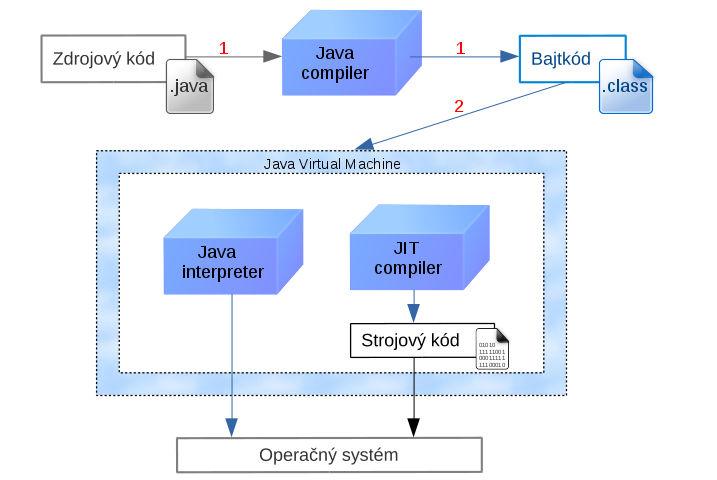
\includegraphics[width=\textwidth]{JVM.png}
  \caption{Grafické znázornenie prekladu a spustenia programu, zdroj: vlastné
  spracovanie}
  \label{fig:jvm}
\end{figure}

\section{Cieľ práce}
TODO...

\section{Členenie práce}
TODO...

\chapter{Bajtkód}
Po preklade zdrojových kódov prekladačom \textit{javac} je každej
triede, prípadne rozhraniu programu priradený jeden \textit{class} súbor
popisujúci jej funkcionalitu.

Pri načítavaní \textit{class} súbru JVM dostane takzvaný prúd inštrukcií
bajtkódu (\textit{bytecode stream}) pre každú metódu triedy. V prípade volania
konkrétnej metódy za behu programu sú inštrukcie danej metódy vykonávané.
Každá z inštrukcí bajtkódu je reprezentovaná číselnou hodnotou nazývanou
\textit{opcode}. Zároveň má každá inštrukcia aj textovú podobu (\textit
{mnemonic}), ktorá je jej menom. V \textit{class} súboorch sú
inštrukcie uložené v numerickej podobe.

Táto kapitola popisuje formát \textit{class} súboru a následne stručne
charakterizuje inštrukčnú sadu bajtkódu.~\footnote{Nasledujúci text vychádza 
zo 4. až 6. kapitoly špecifikácie JVM~\cite{Lindholm:2013:JVM:2462629}.}

\section{Štruktúra \textit{class} súboru}
\textit{Class} súbor pozostáva z jednej \textit{ClassFile} štruktúry. \textit
{ClassFile} štruktúra jednoznačne identifikuje konkrétnu triedu, prípadne
rozhranie, definuje jej premenné a metódy.

Nasledujúci popis definuje sadu datových typov. Typy \textit {u1},
\textit {u2}, a \textit {u4} reprezentujú neznamienkové jedno, dvoj, alebo
štvorbajtové číslo. \textit {ClassFile} je zobrazená ako pseudoštruktúra v
notácií jazyka C. Obsah štruktúry je popísaný ako po sebe nasledujúce položky.

\begin{example}{Formát \textit{ClassFile} štruktúry}
\begin{verbatim}
ClassFile {
  u4 magic;
  u2 minor_version;
  u2 major_version;
  u2 constant_pool_count;
  cp_info constant_pool[constant_pool_count-1];
  u2 access_flags;
  u2 this_class;
  u2 super_class;
  u2 interfaces_count;
  u2 interfaces[interfaces_count];
  u2 fields_count;
  field_info fields[fields_count];
  u2 methods_count;
  method_info methods[methods_count];
  u2 attributes_count;
  attribute_info attributes[attributes_count];
}
\end{verbatim}
\end{example}

Konštanta \textit{magic} identifikuje formát súboru \textit{class},
jej hodnota je 0xCAFEBABE.

Položky \textit{minor\_version} a \textit{major\_version}
určujú verziu \textit{class} súboru. Napríklad \textit{minor\_version} s
hodnotou \textit{m} a \textit{major\_version} s hodnotou \textit{M} indikujú
verziu s hodnotou \textit{M.m}.

Hodnota položky \textit{constant\_pool\_count} je rovná počtu záznamov
v \textit{constant\_pool[]} plus jeden.

Úložisko záznamov \textit{constant\_pool[]} (v podobe poľa štruktúr)
zahŕňa rôzne konštanty: mená tried a rozhraní, mená premenných a iné. Každý
záznam \textit{constant\_pool[]} sa skladá zo značky (\textit{tag}) a indexu
(\textit{name index}). Značka určuje typ záznamu. Tabuľka značiek je uvedená
v prílohe \ref{tab:tab1}. Pomocou unikátneho indexu, je možné odkazovať sa na
záznamy v ďalších častiach bajtkódu. Existuje niekoľko typov
štruktúr~\footnote {Všetky štruktúry \textit{constant\_pool[]} sú popísane v
špecifikácií JVM~\cite{Lindholm:2013:JVM:2462629}.} reprezentujúcich rôzne
druhy záznamov. Napríklad štruktúra \textit{CONSTANT\_String\_info}
reprezentuje objekty typu \textit{String} zatiaľ čo štruktúry
\textit{CONSTANT\_Methodref\_info} a \textit
{CONSTANT\_InterfaceMethodref\_info} reprezentujú metódy danej triedy, alebo
rozhrania.

Hodnota \textit{access\_flags} popisuje oprávnenia prístupu k
informáciam a vlastnosti tejto triedy, respektíve rozhrania pomocou
indikátorov. Napríklad nastavenie indikátora \textit{ACC\_INTERFACE} znamená,
že \textit{class} súbor popisuje rozhranie. Tabuľka indikátorov je uvedená v
prílohe \ref{tab:tab2}.

Položka \textit{this\_class} obsahuje index \textit{constant\_pool[]}
odkazujúci na štruktúru typu \textit{CONSTANT\_Class\_info}~\footnote
{\textit{CONSTANT\_Class\_info} je štrukura \textit{constant\_pool}, ktorá
reprezentuje triedu, alebo rozhranie.}. Reprezentuje triedu, respektíve
rozhranie, definované týmo class súborom.

Hodnotou \textit{super\_class} je taktiež index \textit{constant\_pool[]}
odkazujúci na štruktúru typu \textit{CONSTANT\_Class\_info}. Reprezentuje
priamu nadtriedu triedy definovanej týmto \textit{class} súborom. V prípade,
že tento \textit{class} súbor popisuje rozhranie, index odkazuje na triedu
\textit{Object}. Trieda \textit{Obejct} má ako jediná hodnotu
\textit{super\_class} nulovú.

Počet rozhraní, ktoré trieda implementuje vyjadruje položka
\textit{interface\_count}, v prípade rozhrania je táto položka rovná počtu
priamych nadrozhraní.

Pole \textit{interfaces[]} obsahuje indexy \textit{constant\_pool[]}
odkazujúce na štruktúru typu \textit{CONSTANT\_Class\_info}. Zahŕňa indexy
všetkých rozhraní, ktoré sú implementované triedou, prípadne priamymi
nadrozhraniami \textit{class} súboru.

Položka \textit{fields\_count} je rovná počtu premenných triedy a premenných
inštancí (\textit{fields}) \textit{class} súboru.

Štruktúry typu \textit{field\_info} sú združené v poli \textit{fields[]}. Toto
pole zahŕňa každú premennú danej triedy, respektíve rozhrania. Nezahŕňa
zdedené atribúty. Podrobne sa štruktúrou \textit{field\_info} sa zaoberá
kapitola \ref{sec:fields}.

Hodnata položky \textit{methods\_count} vyjadruje počet štruktúr
\textit{method\_info} v poli \textit{methods[]}.

Položka \textit{methods[]} je pole štruktúr typu \textit{method\_info}. Každá
štruktúra \textit{method\_info} popisuje metódu tejto triedy, respektíve
rozhrania. Zahŕňa konštruktory, metódy triedy a
metód inštancí. Neobsahuje však žiadne zdedené metódy. Štruktúru
\textit{method\_info} popisuje kapitola \ref{sec:methods}.

Hodnota \textit{attributes\_count} je rovná počtu atribútov poľa
\textit{attributes[]} \textit{class} súboru.

Pole \textit{attributes[]} obsahuje štruktúry typu \textit{attribute\_info}.
Atribútmi štruktúry \textit{ClassFile} sú napríklad: \textit{SourceFile},
\textit{Deprecated}, \textit{InnerClasses} a iné. Atribút \textit{SourceFile} 
slúži na reprezentáciu mena \textit{class} súboru. Pole \textit{attributes[]}
\textit{class} súboru môže obsahovať maximálne jeden takýto atribút. Atribút
\textit{Depricated} môže byť použitý v prípade, že bola daná trieda nahradená (\textit{depricated}). Pri volaní takejto triedy môže prekladač upozorníť 
užívateľa, že sa odkazuje na nahradenú triedu~\footnote{Rovnakým spôsobom je možné atribút \textit{Depricated} aplikovať aj na premenné a metódy.}. Vo všeobecnosti sa štruktúre \textit{attribute\_info} sa venuje
kapitola \ref{sec:attributes}.

\subsection{Dátové typy}
\label{sec:descriptors}
Dátové typy sú v \textit{class} súboroch reprezentované vo formáte reťazcov s kódovaním \textit{UTF-8}. Delíme ich na:
\begin{itemize}
\item dátové typy premenných
\begin{itemize}
\item primitívne dátové typy
\item referenčné dátové typy
\item polia
\end{itemize}
\item dátové typy metód
\end{itemize}

Primitívnym dátovým typom (\textit{byte}, \textit{integer}, …) je priradený
popis v podobe znaku (\textit{B}, \textit{I}, …). Napríklad premenná typu
\textit{int} je reprezentovaná znakom: \textit{I}.

Referenčné dátové typy reprezentuje popis v tvare: \textit{L<classname>;}, kde 
\textit{classname} je meno triedy, alebo rozhrania daného referenčného
dátového typu. Premenná typu \textit{Object} je interpretovaná ako
\textit{java/lang/Object;}. 

Identifikačný reťazec jednorozmerného poľa typu \textit{T} sa značí
\textit{[T}, pričom počet znakov \textit{[} je rovný dimenzii poľa. Napríklad
premenná typu: \textit{double d[][][]} generuje reťazec: \textit{[[[D}.

Reťazec dátového typu metódy sa skladá z reťazcov pre dátový typ parametrov,
ohraničených v zátvorkách \textit{(P*)} a reťazca pre dátový typ návratovej
hodnoty \textit{R}. Tvar reťazca dátového typu metódy je potom \textit{(P*)R}.
V prípade návratovej hodnoty \textit{null} je reťazcom návratovej hodnoty znak
\textit{V}. Napríklad metódu \textit{boolean long pow (int n, int k)}
reprezentuje reťazec: \textit{(II)J}, v prípade metódy
\textit{Object method(byte b)} by šlo o reťazec:
\textit{(B)Ljava/lang/Object;}. Komplexný prehľad reprezentácie datových typov
je uvedený v prílohe \ref{tab:tab3}.

\subsection{Premenné tried a inštancií}
\label{sec:fields}
Premenné tried inštancií (\textit{fields}) \textit{class} súboru sú v poli
\textit{fields[]} reprezentované pomocou štruktúry \textit{field\_info}.
Formát štruktúry \textit{field\_info} je nasledovný:

\begin{example}{Štruktúra \textit{field\_info}}
\begin{verbatim}
field_info {
  u2 access_flags;
  u2 name_index;
  u2 descriptor_index;
  u2 attributes_count;
  attribute_info attributes[attributes_count];
}
\end{verbatim}
\end{example}

Položka \textit{access\_flags} je indikátorom oprávnenia prístupu k danej
premennej. Mená indikátorov spolu s ich interpretáciou a hodnotou sú uvedené v
prílohe \ref{tab:tab4}.
     
Dvojbajtová hodnota \textit{name\_index} je index \textit{constant\_pool[]}
reprezentujúci meno premennej

Podobne ako \textit{name\_index} aj \textit{descriptor\_index} je dvojbajtová
položka odkazujúca sa na štruktúru v \textit{constant\_pool}. Na rozdiel od
mena premennej však popisuje datový typ premennej. Reprezentáciou datových
typov sa zaoberá kapitola \ref{sec:descriptors}.

Položka \textit{attributes\_count} vyjadruje počet atribútov v poli
\textit{attributes[]}.

Pole \textit{attributes[]} môže obsahovať ľubovoľné množstvo atribútov
popisujúcich premennú. Štruktúra reprezentujúca atribút je daná všeobecným
predpisom \textit{attributeq\_info}. Atribúty premenných musia byť
reprezentované jednou zo štruktúr \textit{ConstantValue}, \textit{Synthetic},
\textit{Signature}, \textit{Deprecated}, \textit{RuntimeVisibleAnnotations},
alebo \textit{RuntimeInvisibleAnnotations}. Atribút \textit{ConstantValue}
popisuje konštantné statické premenné, \textit{Synthetic} je používaný u
položiek, ktoré sa nevyskytujú v zdrojovom kóde. Štruktúrou
\textit{attribute\_info} sa zaoberá kapitola \ref{sec:attributes}.

\subsection{Metódy}
\label{sec:methods}
Každá metóda triedy, prípadne rozhrania je v poli \textit{methods[]} uložená
pomocou štruktúry \textit{method\_info}. Štruktúra \textit{method\_info} má
nasledujúci formát:

\begin{example}{Štruktúra \textit{method\_info}}
\begin{verbatim}
method_info {
  u2 access_flags;
  u2 name_index;
  u2 descriptor_index;
  u2 attributes_count;
  attribute_info attributes[attributes_count];
}
\end{verbatim}
\end{example}

Indikátor \textit{access\_flags} zahŕňa nastavenia prístupových práv a
vlastností metódy. Tabuľaka indikátorov \textit{access\_flags} štruktúry
\textit{method\_info} sa nachádza v prílohe \ref{tab:tab5}.

Položky \textit{name\_index} a \textit{descriptor\_index} sú podobne ako u
štruktúry \textit{field\_info} indexmi do \textit{constant\_pool}. Tieto indexy
v \textit{constant\_pool} odkazujú na štruktúry popisujúce meno a datový typ
metódy. Reprezentácia dátových typov je popísaná v kapitole
\ref{sec:descriptors}.

Hodnotou položky \textit{attributes\_count} je počet atirbútov
poľa \textit{attributes[}.

Pole \textit{attributes[]} zahŕňa dodatočné atribúty (položky) danej metódy.
Každá položka poľa je reprezentovaná všeobecným predpisom
\textit{attributes\_info}. Počet štruktúr v poli nieje obmedzený, každá
položka však musí byť jednou zo štruktúr: \textit{Code}, \textit{Exceptions},
\textit{Synthetic},\textit{Signature}, \textit{Deprecated},
\textit{RuntimeVisibleAnnotations}, \textit{RuntimeInvisibleAnnotations},
\textit{RuntimeVisibleParameterAnnotations},
\textit{RuntimeInvisibleParameterAnnotations},
alebo \textit{AnnotationDefault}.
Atribút \textit{Code} je jedným z najdôležitejších. Obshauje inštrukcie
bajtkódu popisujúce fungovanie metódy. Okrem metód deklarovaných ako
abstraktná, alebo natívna musí každá metóda obsahovať práve jeden atribút
\textit{Code}. Atribút \textit{Exceptions} zahŕňa indexy výnimiek, ktoré
metóda vyhadzuje. Popisom formátu štruktúry \textit{attributes\_info} sa
zaoberá kapitola \ref{sec:attributes}.

\subsection{Atribúty}
\label{sec:attributes}
Pojem atribút v tomto texte vyjadruje atribúty používané v poli
\textit{attributes[]} štruktúr \textit{field\_info}, \textit{method\_info} a
\textit{Code\_attributes}. Všeobecný predpis všetkých atribútov je vyjadrený
štruktúrou \textit{attribute\_info}. Existuje niekoľko základných
preddefinovaných atribútov: \textit{SourceFile}, \textit{ConstantValue},
\textit{Code}, \textit{Exceptions}, \textit{InnerClasses}, \textit{Synthetic},
\textit{LineNumberTable}, \textit{LocalVariableTable}, \textit{Deprecated} a
iné. Líšia sa funkcionalitou a využitím jednotlivými časťami \textit{class}
súboru. Všetky atribúty vychádzajú z už spomínaného všeobecného predpisu
\textit{attribute\_info}, ktorý má nasledujúci formát:

\begin{example}{Štruktúra \textit{attribute\_info}}
\begin{verbatim}
attribute_info {
  u2 attribute_name_index;
  u4 attribute_length;
  u1 info[attribute_lenght];
}
\end{verbatim}
\end{example}

Položka \textit{attributes\_name\_index} je indexom do \textit{constant\_pool}odkazujúcim na meno atribútu.

Štvorbajtová položka \textit{attribute\_length} je rovná hodnote vyjadrujúcej
dĺžku následných informácií uložených v \textit{info[attribute\_length]}.
Informácie sa líšia na základe odlišnej funkcionality a využitá jednotlivých
atribútov.

\section{Inštrukčná sada bajtkódu}
TODO...

\clearpage
\addcontentsline{toc}{chapter}{Literatúra} 
\bibliographystyle{alpha} 
\bibliography{bp} 

\appendix

\chapter{Tabuľky}
Zdrojom nasledujúcich tabuliek je špecifikácia JVM
JVM~\cite{Lindholm:2013:JVM:2462629}.

\begin{table}
  \begin{tabular}{| l | c |}
    \hline
    \textbf{Constant Type} & \textbf{Value} \\
    \hhline{|=|=|}
    CONSTANT\_Class & 7 \\ \hline
    CONSTANT\_Fieldref & 9 \\ \hline
    CONSTANT\_Methodref & 10 \\ \hline
    CONSTANT\_InterfaceMethodref & 11 \\ \hline
    CONSTANT\_String & 8 \\ \hline
    CONSTANT\_Integer & 3 \\ \hline
    CONSTANT\_Float & 4 \\ \hline
    CONSTANT\_Long & 5 \\ \hline
    CONSTANT\_Double & 6 \\ \hline
    CONSTANT\_NameAndType & 12 \\ \hline
    CONSTANT\_Utf8 & 1 \\ \hline
    CONSTANT\_MethodHandle & 15 \\ \hline
    CONSTANT\_MethodType & 16 \\ \hline
    CONSTANT\_InvokeDynamic & 18 \\
    \hline
  \end{tabular}
  \caption{Tabuľka značiek určujúcich typ záznamu v \textit{constant\_pool}.
  Stĺpec \textit{Constant Type} označuje názov typu, stĺpec \textit{value}
  priraďuje každému typu číselnú hodnotu.}
  \label{tab:tab1}
\end{table}

\begin{table}
  \begin{tabular}{| l | c | p{6cm} |}
    \hline
    \textbf{Meno Indikátora} & \textbf{Hodnota} & \textbf{Interpretácia} \\
    \hhline{|=|=|=|}
    ACC\_PUBLIC & 0x0001 & Deklarovaná ako verejná; prístupná aj mimo balíka.
    \\ \hline
    ACC\_FINAL & 0x0010 & Deklarovaná ako final; žiadne podtriedy po 
    inicializácií. \\ \hline
    ACC\_SUPER & 0x0020 & Volá metódu nadtriedy, hlavne inštrukcia 
    invokespecial. \\ \hline
    ACC\_INTERFACE & 0x0200 & Je rozhranie, nie trieda.\\ \hline
    ACC\_ABSTRACT & 0x0400 & Deklarovaná ako abstraktná, nemôže byť 
    inštanciovaná. \\ \hline
    ACC\_SYNTHETIC & 0x1000 & Deklarovaná ako synthetic, nieje prítomná v 
    zdrojovom kóde. \\ \hline
    ACC\_ANNOTATION & 0x2000 & Deklarovaná ako typ annotation. \\ \hline
    ACC\_ENUM & 0x4000 & Deklarovaná ako typ enum. \\    
    \hline
  \end{tabular}
  \caption{Tabuľka indikátorov prístupových práv \textit{ClassFile} štruktúry.}
  \label{tab:tab2}
\end{table}

\begin{table}
  \begin{tabular}{| p{3cm} | c | p{6,5cm} |}
    \hline
    \textbf{Reprezentácia pomocou reťazca} & \textbf{Typ} & 
    \textbf{Interpretácia} \\
    \hhline{|=|=|=|}
     B & byte &  znamienkové celé číslo veľkosti jedného bajtu \\ \hline
     C & char & Znak s kódovaním UTF-16 \\ \hline
     D & double & číselná hodnota s dvojitou presnosťou a plávajúcou
     desatinnou čiarkou \\ \hline
     F & float & číselná hodnota s plávajúcou desatinnou čiarkou \\ \hline
     I & int & celé číslo \\ \hline
     J & long & celé číslo väčšieho rozsahu \\ \hline
     L ClassName ; & referencia & inštancia triedy ClassName \\ \hline
     S & short & znamienkové celé číslo krátkeho rozsahu \\ \hline
     Z & boolean & pravda alebo nepravda \\ \hline
     [ & reference & jednorozmerné pole \\
    \hline
  \end{tabular}
  \caption{Tabuľka reprezentácie datových typov pre premenné.}
  \label{tab:tab3}
\end{table}

\begin{table}
  \begin{tabular}{| l | c | p{6,5cm} |}
    \hline
    \textbf{Meno Indikátora} & \textbf{Hodnota} & \textbf{Interpretácia} \\
    \hhline{|=|=|=|}
    ACC\_PUBLIC & 0x0001 & Deklarovaná ako verejná; prístupná aj mimo balíka.
    \\ \hline
    ACC\_PRIVATE & 0x0002 & Deklarovaná ako privátna; použiteľná len vrámci 
    triedy, v ktorej bola definovaná. \\ \hline
    ACC\_PROTECTED & 0x0004 & Deklarovaná ako protected; prístupná aj 
    podtriedam. \\ \hline
    ACC\_STATIC & 0x0008 & Deklarovaná ako statická. \\ \hline
    ACC\_FINAL & 0x0010 & Deklarovaná ako final; žiadne ďalšie priradenia po
    inicializácií. \\ \hline
    ACC\_VOLATILE & 0x0040 & Deklarovaná ako volatile; nemôže byť uložená do medzipamäte. \\ \hline
    ACC\_TRANSIENT & 0x0080 & Deklarovaná ako transient; nieje čítaná ani
    modifikovaná objektovým manažérom. \\ \hline
    ACC\_SYNTHETIC & 0x1000 & Deklarovaná ako synthetic, nieje prítomná v zdrojovom kóde. \\ \hline
    ACC\_ENUM & 0x4000 & Deklarovaná ako prvok objektu enum \\
    \hline
  \end{tabular}
  \caption{Tabuľka indikátorov prístupových práv a vlastností štruktúry
  \textit {field\_info}.}
  \label{tab:tab4}
\end{table}

\begin{table}
  \begin{tabular}{| l | c | p{5,5cm} |}
    \hline
    \textbf{Meno Indikátora} & \textbf{Hodnota} & \textbf{Interpretácia} \\
    \hhline{|=|=|=|}
    ACC\_PUBLIC & 0x0001 & Deklarovaná ako verejná; prístupná aj mimo balíka.
    \\ \hline
    ACC\_PRIVATE & 0x0002 & Deklarovaná ako privátna; použiteľná len vrámci 
    triedy, v ktorej bola definovaná. \\ \hline
    ACC\_PROTECTED & 0x0004 & Deklarovaná ako protected; prístupná aj 
    podtriedam. \\ \hline
    ACC\_STATIC & 0x0008 & Deklarovaná ako statická. \\ \hline
    ACC\_FINAL & 0x0010 & Deklarovaná ako final; nemôže byť prepísaná.
    \\ \hline
    ACC\_SYNCHRONIZED & 0x0020 & Deklarovaná ako synchronized; pri volaní je
    zabalená za použitia monitora. \\ \hline
    ACC\_BRIDGE & 0x0040 & Bridge metóda; je generovaná prekladačom. \\ \hline
    ACC\_VARARGS & 0x0080 & Deklarovaná s dynamickým počtom argumentov.
    \\ \hline
    ACC\_NATIVE & 0x0100 & Deklarovaná ako natívna; implementovaná v inom jazyku ako Java.
    \\ \hline
    ACC\_ABSTRACT & 0x0400 & Deklarovaná ako abstraktná, nieje implementovaná. \\ \hline
    ACC\_STRICKT & 0x0800 & Deklarovaná ako stricktfp, výpočty s plávajúcou
    čiarkou sú FP - strict. \\ \hline
    ACC\_SYNTHETIC & 0x1000 & Deklarovaná ako synthetic, nieje prítomná v zdrojovom kóde. \\
    \hline
  \end{tabular}
  \caption{Tabuľka indikátorov prístupových práv a vlastností štruktúry
  \textit {method\_info}.}
  \label{tab:tab5}
\end{table}

\end{document}